\chapter{Erste Schritte}
\label{kap:erste-schritte}

Dieses Kapitel führt einmal durch die wichtigsten Arbeitsschritte: eine
Schaltung anlegen, simulieren, Werte ändern, einen Frequenzgang mit
Grenzfrequenz bestimmen, im Plan zeichnen und eine Parameterstudie rechnen.
Am Ende steht dieselbe Simulation einmal auf der Kommandozeile. Wer die
Schritte nachvollzieht, kennt danach den Großteil der täglichen Arbeit.

\section{Eine neue Schaltung}

Nach dem Start zeigt der Editor ein leeres Fenster.
\menue{Datei}\pfad\menue{Neu} (\tasten{Strg}{N}) legt eine Vorlage an: einen
RC-Tiefpass aus einer Pulsquelle \code{V1}, einem Widerstand \code{R1} und
einem Kondensator \code{C1}.

Das Fenster hat drei große Bereiche (Abbildung~\ref{abb:tiefpass}):

\begin{itemize}
  \item in der Mitte der \textbf{Schaltplan},
  \item rechts der \textbf{Text} der Datei, also die Eingabe für den
    Simulator,
  \item unten die \textbf{Ergebnisse}, daneben als Reiter das
    \textbf{Protokoll} und die Liste der \textbf{Probleme},
  \item links die Listen \textbf{Bauteile} und \textbf{Eigenschaften}.
\end{itemize}

\begin{figure}[htbp]
  \centering
  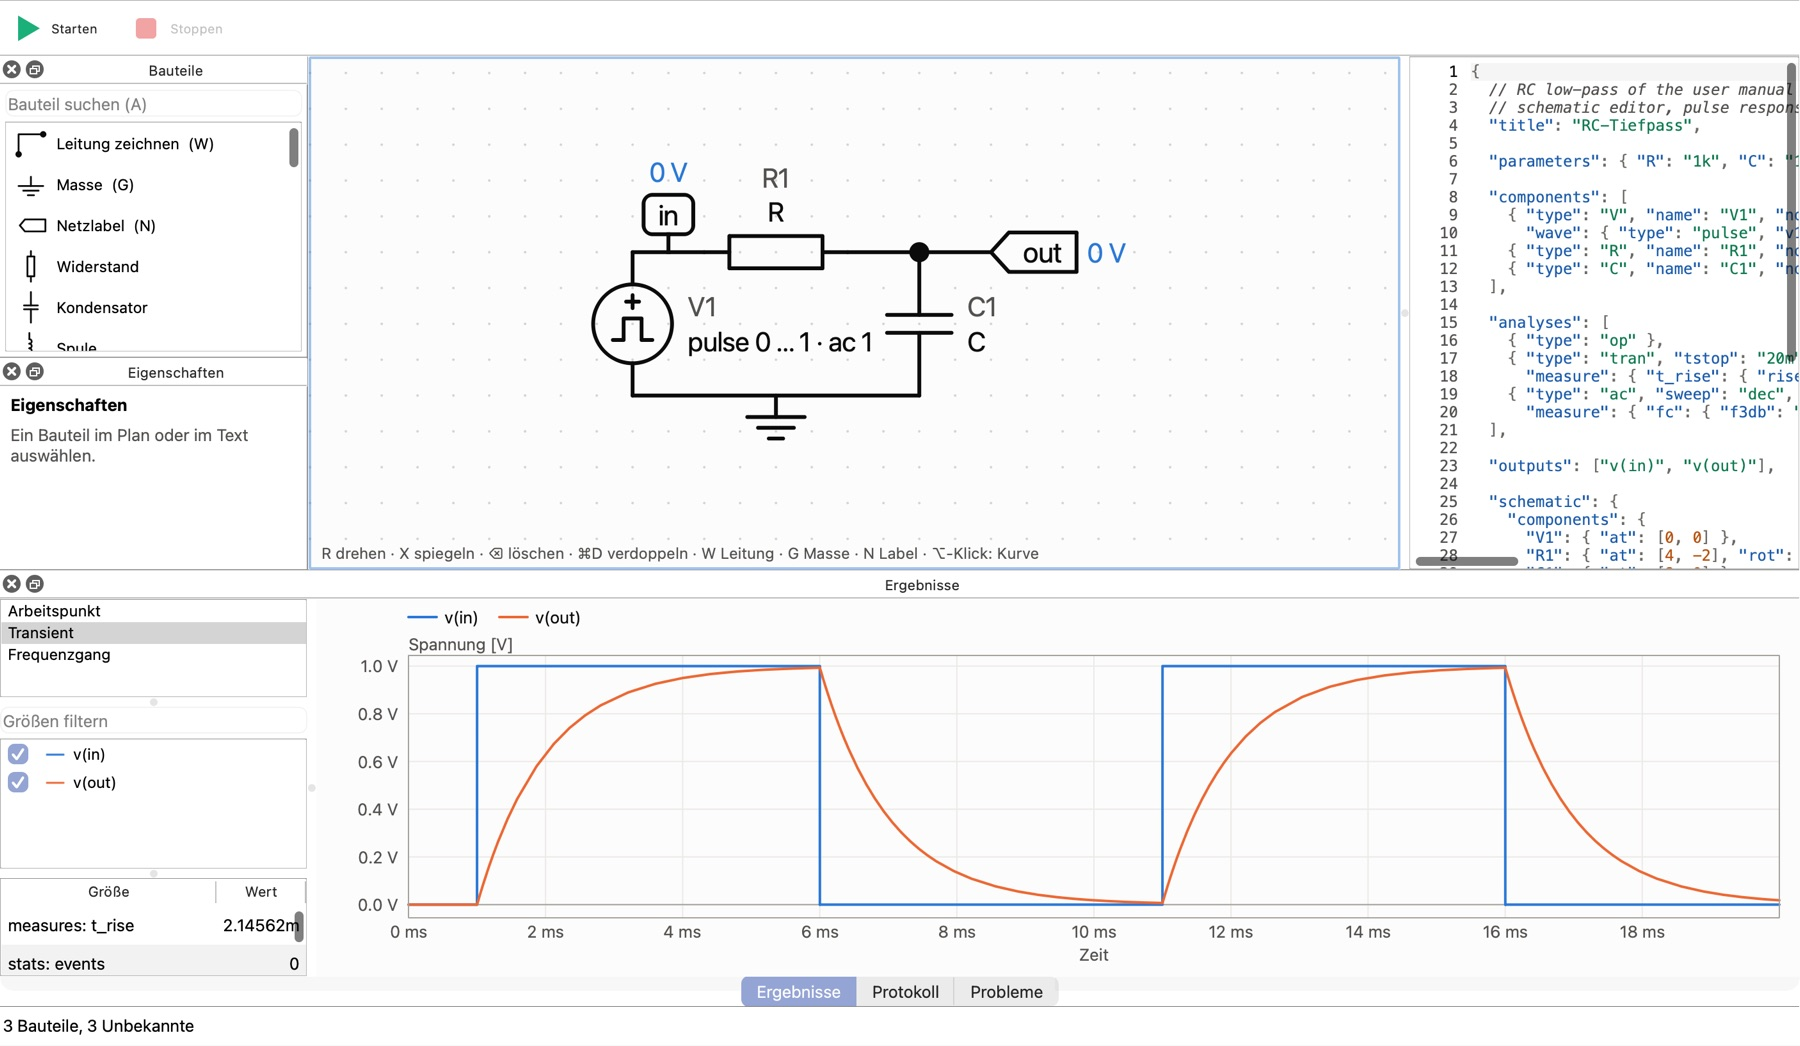
\includegraphics[width=\textwidth]{tiefpass.jpg}
  \caption{Der RC-Tiefpass im Editor: Plan, Text und Sprungantwort. Die
    Datei liegt als \code{docs/handbuch/tiefpass.json} bei.}
  \label{abb:tiefpass}
\end{figure}

Plan und Text sind zwei Ansichten derselben Datei. Ein Klick auf \code{R1}
im Plan markiert dessen Zeile im Text; setzt man den Textcursor in die
Zeile von \code{C1}, wird \code{C1} im Plan ausgewählt. Jede Änderung im
Plan erscheint sofort im Text und umgekehrt.

\section{Die erste Simulation}

\menue{Simulation}\pfad\menue{Starten} oder \tasten{Strg}{R} startet die
Rechnung. Der Simulator liest die Datei von der Platte; deshalb sichert der
Editor vorher ungesicherte Änderungen, und eine Datei ohne Namen fragt nach
einem Speicherort. Während der Rechnung zeigt
die Statuszeile den Fortschritt; \tasten{Strg}{.} bricht ab.

Danach steht im Ergebnisfeld links die Liste der Analysen der Datei:
\menue{Arbeitspunkt} und \menue{Transient}. Ein Klick auf
\menue{Transient} zeigt den Zeitverlauf: die Pulsspannung \code{v(in)} und
die Kondensatorspannung \code{v(out)}, die mit der Zeitkonstante
$\tau = RC = 1\,\text{ms}$ folgt. Mit den Häkchen unter \menue{Größen
filtern} werden Kurven ein- und ausgeblendet.

Im Kurvenfeld:
\begin{itemize}
  \item Mausrad oder Spreizen auf dem Touchpad zoomt in $x$, mit
    \taste{Strg} in $y$,
  \item Ziehen mit der Maus zoomt auf ein Rechteck,
  \item Doppelklick (oder \tasten{Strg}{0}) zeigt wieder alles,
  \item das Fadenkreuz folgt der Maus und zeigt die Werte aller Kurven.
\end{itemize}

Im Plan stehen jetzt an den Netzlabels die Spannungen des Arbeitspunkts
(hier 0\,V, weil die Pulsquelle bei $t=0$ auf 0\,V steht).

\section{Werte ändern}

Ein Klick auf \code{R1} zeigt unter \menue{Eigenschaften} ein Formular mit
Name, Anschlüssen und allen Werten des Bauteils. Dort \code{value} auf
\code{2.2k} setzen und mit der Eingabetaste bestätigen. Im Text steht
sofort \code{"value": "2.2k"}. Nach \tasten{Strg}{R} steigt \code{v(out)}
deutlich langsamer.

Genauso gut lässt sich der Wert direkt im Text ändern. Der Editor prüft
die Datei beim Tippen mit dem Parser des Simulators: Ein Tippfehler wie
\code{"valeu"} erscheint sofort als Warnung an der Zeile und in der Liste
\menue{Probleme}; ein Doppelklick dort springt an die Stelle.

\begin{hinweis}
  Zahlen dürfen SI-Präfixe tragen: \code{2.2k}, \code{100n}, \code{4.7meg}.
  Groß- und Kleinschreibung zählt – \code{M} ist Mega, \code{m} Milli
  (Abschnitt~\ref{sec:zahlen}).
\end{hinweis}

\section{Frequenzgang und Grenzfrequenz}

Für einen Frequenzgang braucht die Quelle eine Kleinsignalamplitude und die
Datei eine AC-Analyse. In den Eigenschaften von \code{V1} in der letzten
Zeile \menue{Neu} den Namen \code{ac} und den Wert \code{1} eintragen und
mit \taste{+} übernehmen. Dann im Text unter \code{"analyses"} eine Zeile
ergänzen:

\begin{json}
"analyses": [
  { "type": "op" },
  { "type": "tran", "tstop": "20m" },
  { "type": "ac", "sweep": "dec", "points": 20, "fstart": 1, "fstop": "100k",
    "measure": { "fc": { "f3db": "v(out)" } } }
],
\end{json}

Nach \tasten{Strg}{R} zeigt \menue{Frequenzgang} Betrag (in dB) und Phase
über der Frequenz. Die Messgröße \code{fc} steht in der Wertetabelle unter
der Liste der Größen: rund 159\,Hz für 1\,k\ohm\ und 1\,µF, wie
$f_c = 1/(2\pi RC)$ erwarten lässt.

\section{Im Plan zeichnen}

Nun soll eine zweite RC-Stufe an \code{out} angehängt werden.

\begin{enumerate}
  \item \textbf{Widerstand platzieren.} \taste{A} drücken (oder in die
    Liste \menue{Bauteile} klicken), »wid« tippen, Eingabetaste. Am
    Mauszeiger hängt jetzt ein Widerstand. \taste{R} dreht ihn um 90°,
    \taste{X} spiegelt ihn. Ein Klick setzt ihn ab; der nächste Klick setzt
    einen weiteren. \taste{Esc} beendet das Platzieren.
  \item \textbf{Kondensator platzieren} auf dieselbe Weise (»kon«).
  \item \textbf{Leitungen ziehen.} \taste{W} startet eine Leitung. Ein Klick
    setzt den Anfang, jeder weitere Klick eine Ecke. Die Leitung knickt
    rechtwinklig; \taste{/} wählt, ob sie zuerst waagrecht oder zuerst
    senkrecht verläuft. Sie endet von selbst, sobald ein Klick einen
    Anschluss oder eine andere Leitung trifft; sonst beendet ein Doppelklick
    oder \taste{Esc} sie. \taste{Entf} nimmt die letzte Ecke zurück.
  \item \textbf{Masse.} \taste{G} hängt ein Massesymbol an den Mauszeiger;
    ein Klick auf das freie Ende des Kondensators setzt es.
  \item \textbf{Netzlabel.} \taste{N} fragt nach einem Namen, z.\,B.
    \code{out2}, und setzt das Label per Klick an die neue Leitung.
\end{enumerate}

Der Text enthält danach zwei neue Bauteile \code{R2} und \code{C2} mit den
Knoten, die der Plan vorgibt: \code{["out", "out2"]} und
\code{["out2", "0"]}. Knotennamen entstehen aus den Labels; Netze ohne Label
bekommen Namen wie \code{n1}. Wer \code{v(out2)} als Kurve sehen will,
ergänzt es unter \code{"outputs"} – oder klickt nach der Simulation mit
gedrückter \taste{Alt}-Taste auf die Leitung.

\begin{hinweis}[Alt-Klick]
  Ein Klick mit \taste{Alt} auf eine Leitung zeigt deren Spannung, auf ein
  Bauteil dessen Strom als Kurve. Ist die Größe nicht unter
  \code{"outputs"} gespeichert, sagt die Statuszeile, was einzutragen ist.
\end{hinweis}

Ausgewählte Bauteile verschiebt man durch Ziehen oder mit den Pfeiltasten
(mit \taste{Umschalt} in Fünferschritten); angeschlossene Leitungen gehen
mit. \tasten{Strg}{D} verdoppelt die Auswahl, \taste{Entf} löscht sie,
\tasten{Strg}{Z} nimmt jeden Schritt zurück – auch Änderungen im Text,
denn Plan und Text haben eine gemeinsame Undo-Geschichte.

\section{Parameter und eine Parameterstudie}

Statt fester Werte können Bauteile Parameter verwenden. Im Text:

\begin{json}
"parameters": { "R": "1k", "C": "1u" },
"components": [
  ...
  { "type": "R", "name": "R1", "nodes": ["in", "out"], "value": "R" },
  { "type": "C", "name": "C1", "nodes": ["out", "0"], "value": "C" }
],
\end{json}

Eine Analyse lässt sich nun für mehrere Werte eines Parameters wiederholen:

\begin{json}
{ "type": "tran", "tstop": "20m",
  "param_sweep": { "param": "C", "values": ["470n", "1u", "2.2u"] } }
\end{json}

Das Ergebnis zeigt eine Kurvenschar: eine Farbstufe je Wert. Messgrößen
einer Studie lassen sich zusätzlich als Kennlinie über dem Parameter
darstellen (Kapitel~\ref{kap:editor-ergebnisse}).

\section{Sichern und auf der Kommandozeile rechnen}

\tasten{Strg}{S} sichert die Datei. Sie enthält alles: Bauteile, Modelle,
Analysen und unter \code{"schematic"} den Plan. Dieselbe Datei rechnet der
Simulator ohne Editor:

\begin{shell}
esim tiefpass.json -o ergebnisse
\end{shell}

\begin{shell}
RC-Tiefpass
3 components, 3 unknowns (2 node voltages, 1 branch currents, 0 equation variables)
[op] converged after 1 iterations (newton)
  v(in)  = 0
  v(out) = 0
[tran] 0 .. 0.02 s, bdf (order up to 5): 160 steps ... -> ergebnisse/tiefpass.tran.csv
  t_rise = 0.00214562
[ac] 1 .. 100000 Hz: 101 points -> ergebnisse/tiefpass.ac.csv
  fc = 159.182
\end{shell}

Die Kurven liegen als CSV-Dateien im Ordner \datei{ergebnisse}, eine je
Analyse. Wie es von hier weitergeht, beschreiben Teil~II (Editor) und
Teil~III (alle Möglichkeiten der Eingabedatei).
